\documentclass[tikz]{standalone}

\usepackage{amsmath}
\usepackage{lmodern}
\usepackage{pgfplots}
\usepackage{physics}

\pgfplotsset{compat=1.17}

\usetikzlibrary{arrows.meta}

\definecolor{exotic orange}{RGB}{255,128,0}
\definecolor{exotic green}{RGB}{0,102,102}
\definecolor{exotic blue}{RGB}{67,132,161}
\definecolor{exotic red}{RGB}{250,86,86}

\begin{document}
	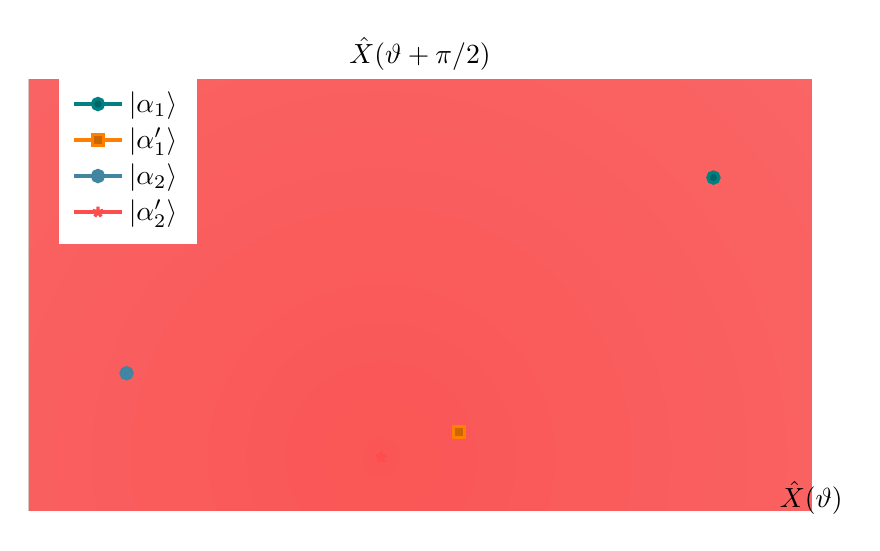
\begin{tikzpicture}
		\begin{axis}[
			width=0.95\linewidth,
			axis lines=center,
			axis equal image,
			xlabel={$\hat{X}(\vartheta)$},
			ylabel={$\hat{X}(\vartheta+\pi/2)$},
			ticks=none,
			xmin=-2,
			xmax=+2,
			ymin=-0.2,
			ymax=+2,
			axis line style={thick},
			x label style={
				anchor=north,
			},
			y label style={
				anchor=south,
			},
			cycle list name=exotic,
				legend style={
					at={(axis cs: -1,1.6)},
					anchor=east,
					draw=none,
					inner sep=5,
					outer sep=10,
				},
			legend cell align={left},
		]
			\draw[thick, -Latex, dotted, gray] (axis cs:1.3,1.3) -- (axis cs:0.4,0.4);
			\draw[thick, -Latex, dotted, gray] (axis cs:-1.3,0.4) -- (axis cs:-0.4,0.15);
		
			\addplot+[very thick] coordinates {(1.5,1.5)};
			\shadedraw[inner color=exotic green, outer color=exotic green!40, draw=none] (axis cs:1.5,1.5) circle (20);
			
			\addplot+[very thick] coordinates {(0.2,0.2)};
			\shadedraw[inner color=exotic orange, outer color=exotic orange!40, draw=none] (axis cs:0.2,0.2) circle (20);
			
			\addplot+[very thick] coordinates {(-1.5,0.5)};
			\shadedraw[inner color=exotic blue, outer color=exotic blue!40, draw=none] (axis cs:-1.5,0.5) circle (20);
			
			\addplot+[very thick] coordinates {(-0.2,0.07)};
			\shadedraw[inner color=exotic red, outer color=exotic red!40, draw=none] (axis cs:-0.2,0.07) circle (20);
			
			\legend{$\ket{\alpha_1}$,$\ket{\alpha_1^\prime}$,$\ket{\alpha_2}$,$\ket{\alpha_2^\prime}$};
		\end{axis}
	\end{tikzpicture}
\end{document}